\documentclass{VUMIFPSbakalaurinis}
\usepackage{float}
\usepackage{hyperref}
\usepackage{algorithmicx}
\usepackage{algorithm}
\usepackage{algpseudocode}
\usepackage{amsfonts}
\usepackage{amsmath}
\usepackage{bm}
\usepackage{caption}
\usepackage{color}
\usepackage{graphicx}
\usepackage{listings}
\usepackage{subcaption}
\usepackage{wrapfig}
\usepackage{biblatex}
\usepackage{microtype}

% Titulinio aprašas
\university{Vilniaus universitetas}
\faculty{Matematikos ir informatikos fakultetas}
\institute{Informatikos institutas}  % Užkomentavus šią eilutę - institutas neįtraukiamas į titulinį
\department{Programų sistemų bakalauro studijų programa}
\papertype{Bakalauro baigiamojo darbo planas}
\title{Monolitų migravimas naudojant dekomponavimą pagal domenus ir „Mono2Micro”}
\titleineng{Migrating a monolith using domain driven design and "Mono2Micro"}
\author{Audrius Kumpis}
% \secondauthor{Vardonis Pavardonis}   % Pridėti antrą autorių
\supervisor{lekt. Vasilij Savin}
% \reviewer{doc. dr. Vardauskas Pavardauskas}
\addsignatureplaces{} % prideda parašų vietas tituliniame puslapyje
\date{Vilnius – \the\year}

\bibliography{bibliografija}

\begin{document}
\maketitle

\sectionnonum{Darbo planas}
Kai komanda pradeda kurti programą, monolitas įprastai yra numatytas pasirinkimas. Tai yra viena pagrindinių priežasčių, kodėl egzistuoja itin daug monolitinių sistemų. Monolitas turi savo duomenų bazę, savo funkcionalumo įgyvendinimą ir tai yra vientisa programa. Jis yra lengvai suprogramuojamas ir su palyginamai nedideliu darbo indėliu, galima greitai sukurti bei diegti veikiančią sistemą. Tačiau tokią architektūrą yra labai sunku plėtoti bei palaikyti. Kuo daugiau  tokia sistema yra plėtojama, tuo daugiau ji didėja, daugėja kodo bei priklausomybių nuo kitų sistemų. Diegimai tampa ilgi ir itin reti. Testavimas būna sudėtingas, nes negalima atlikti izoliuoto atskirų sistemos modulių testavimo. Kad ši problema būtų išspręsta, paprastai monolitinės sistemos yra skaidomos į mikroservisus.

Mikroservisai – tai atskiri, nedideli servisai, kurie atsakingi už tam tikras specifines užduotis. Jie yra implementuoti kaip atskiros programos, o komunikacija tarp jų įprastai yra vykdoma per pranešimų siuntimo (angl. messaging) technologijas arba per REST API. Kiekvienas mikroservisas turi savo duomenų bazę, savo diegimo strategijas bei testavimo aplinką. Mikroservisų architektūra suteikia daug privalumų, pavyzdžiui:
\begin{itemize}
    \item Pagreitinami sistemos diegimai.
    \item Pagerinamas sistemos plečiamumas.
    \item Nėra priklausomybės nuo pasirinktų technologijų.
    \item Prie sistemos implementacijos gali dirbti didesnis komandų skaičius.
\end{itemize}

Nors mikroservisai išsprendžia daug problemų, tai nėra paprastas sprendimas. Kadangi migravimas į mikroservisų architektūrą yra pilnai techninė užduotis, privaloma gauti projekto vadovo ir/ar projekto savininko sutikimą, kad migracijai būtų skiriami resursai bei lėšos. Viena iš sunkesnių migracijos dalių yra mikroservisų projektavimas. Yra daugybė būdų, kaip galima išskaidyti monolitinę sistemą į mažesnius servisus \cite{FBZ+19}, taigi iš anksto apgalvoti, kokia strategija bus taikoma yra svarbu ir laiko, ir resursų atžvilgiu. Kad migracija iš monolitinės architektūros į mikroservisų būtų sklandi, reikia gerai žinoti, kokius darbus ir kokia tvarka būtina atlikti. Jau egzistuoja keletas migravimo atlikimo strategijų \cite{Wal22,MQO18,KXL+20}, su kuriomis susipažinus yra lengviau suplanuoti reikiamus darbus. Šiame darbe bus aptartos šios strategijos:
\begin{itemize}
    \item Dekomponavimas skaidant domenus.
    \item Visiškas sistemos perdarymas.
    \item Dekomponavimas naudojant dirbtiniu intelektu paremtą įrankį „Mono2Micro“.
\end{itemize}

\sectionnonum{Darbo tikslas ir uždaviniai}
Darbo tikslas: atlikti tyrimą nagrinėjant „Mono2Micro“ techninės galimybės ir galimą naudą, įskaitant pagerintą mastelio keitimą, lankstumą ir priežiūrą. Tyrimo tikslas - nustatyti pagrindinius veiksnius, turinčius įtakos migravimo proceso sėkmei, įvertinti šio metodo našumą, bei pateikti rekomendacijas organizacijoms, svarstančioms apie šio įrankio panaudojimą. Taip pat šio tyrimo tikslas yra prisidėti prie augančio žinių apie mikroservisų architektūrą kiekio ir pateikti praktinių įžvalgų informacinių technologijų specialistams, dalyvaujantiems programinės įrangos modernizavimo iniciatyvose.

Tyrimo tikslams pasiekti bus atliekamos kelios užduotys. Pirma, bus analizuojama monolitinė programa, siekiant nustatyti jos pagrindines funkcijas ir priklausomybes. Antra, bus naudojamas įrankis „Mono2Micro“, kad monolitinė programa būtų migruojama į mikroservisus, remiantis domenais orientuoto projektavimo principais. Trečia, sukurtos mikroservisų architektūros našumas, masteliškumas ir palaikomumas bus vertinamas pagal tokius rodiklius, kaip atsako laikas, pralaidumas ir išteklių naudojimas.

Siekiant įvertinti migracijos metodo veiksmingumą, bus naudojami minėti našumo rodikliai, kad būtų galima palyginti monolitinės taikomosios programos ir sukurtos mikroservisų architektūros našumą. Architektūros judrumas bus vertinamas pagal jos gebėjimą reaguoti į besikeičiančius verslo reikalavimus ir jos diegimo bei mastelio keitimo paprastumą. Architektūros masteliškumas bus vertinamas pagal jos gebėjimą susidoroti su didėjančiomis apkrovomis ir gebėjimą masteliuoti horizontaliai ir vertikaliai.
% Nurodomi iki 5 svarbiausių temos raktinių žodžių (terminų).
% Vienas terminas gali susidėti iš kelių žodžių.
% \raktiniaizodziai{raktinis žodis 1, raktinis žodis 2, raktinis žodis 3, raktinis žodis 4, raktinis žodis 5}   

% \sectionnonumnocontent{Summary}
% Santrauka anglų kalba. Santraukos apimtis ne didesnė nei 0,5 puslapio.
% \keywords{keyword 1, keyword 2, keyword 3, keyword 4, keyword 5}

% \tableofcontents

% \sectionnonum{Įvadas}
% Įvade nurodomas darbo tikslas ir uždaviniai, kuriais bus įgyvendinamas tikslas,
% aprašomas temos aktualumas, apibrėžiamas tiriamasis objektas akcentuojant
% neapibrėžtumą, kuris bus išspręstas darbe, aptariamos teorinės darbo prielaidos
% bei metodika, apibūdinami su tema susiję literatūros ar kitokie šaltiniai,
% temos analizės tvarka, darbo atlikimo aplinkybės, pateikiama žinių apie
% naudojamus instrumentus (programas ir kt., jei darbe yra eksperimentinė dalis).
% Darbo įvadas neturi būti dėstymo santrauka. Įvado apimtis 2--4 puslapiai.

% \section{Medžiagos darbo tema dėstymo skyriai}
% Medžiagos darbo tema dėstymo skyriuose išsamiai pateikiamos nagrinėjamos temos
% detalės: pradiniai duomenys, jų analizės ir apdorojimo metodai, sprendimų
% įgyvendinimas, gautų rezultatų apibendrinimas.

% Medžiaga turi būti dėstoma aiškiai, pateikiant argumentus. Tekste dėstomas
% trečiuoju asmeniu, t.y. rašoma ne \enquote{aš manau}, bet „autorius mano“, „autoriaus
% nuomone“. Reikėtų vengti informacijos nesuteikiančių frazių, pvz., „...kaip jau
% buvo minėta...“, „...kaip visiems žinoma...“ ir pan., vengti grožinės
% literatūros ar publicistinio stiliaus, gausių metaforų ar panašių meninės
% išraiškos priemonių.

% Skyriai gali turėti poskyrius ir smulkesnes sudėtines dalis, kaip punktus ir
% papunkčius.

% \subsection{Poskyris}
% Citavimo pavyzdžiai: cituojamas vienas šaltinis \cite{PvzStraipsnLt}; cituojami
% keli šaltiniai \cite{PvzStraipsnEn, PvzKonfLt, PvzKonfEn, PvzKnygLt, PvzKnygEn,
% PvzElPubLt, PvzElPubEn, PvzMagistrLt, PvzPhdEn}.

% \subsection{Faktorialo algoritmas}

% \ref{alg:factorial} pav. pateiktas faktorialo algoritmas.

% \begin{algorithm}
% \begin{algorithmic}[1] % [1] padaro, kad eilutės būtų sunumeruotos
% \State $N\gets$ skaičius, kurio faktorialą skaičiuojame
% \State $F\gets 1$
% \For{$i := 2$ $to$ $N$}
%     \State $F\gets F \cdot i$
% \EndFor
% \end{algorithmic}
% \caption{Faktorialo algoritmas}
% \label{alg:factorial}
% \end{algorithm}

% \subsubsection{Punktas}
% \subsubsubsection{Papunktis}
% \subsubsection{Punktas}
% \section{Skyrius}
% \subsection{Poskyris}
% \subsection{Poskyris}

% \sectionnonum{Rezultatai ir išvados}
% Rezultatų ir išvadų dalyje išdėstomi pagrindiniai darbo rezultatai (kažkas
% išanalizuota, kažkas sukurta, kažkas įdiegta), toliau pateikiamos išvados
% (daromi nagrinėtų problemų sprendimo metodų palyginimai, siūlomos
% rekomendacijos, akcentuojamos naujovės). Rezultatai ir išvados pateikiami
% sunumeruotų (gali būti hierarchiniai) sąrašų pavidalu. Darbo rezultatai turi
% atitikti darbo tikslą.

\printbibliography[heading=bibintoc]  % Šaltinių sąraše nurodoma panaudota
% literatūra, kitokie šaltiniai. Abėcėlės tvarka išdėstomi darbe panaudotų
% (cituotų, perfrazuotų ar bent paminėtų) mokslo leidinių, kitokių publikacijų
% bibliografiniai aprašai. Šaltinių sąrašas spausdinamas iš naujo puslapio.
% Aprašai pateikiami netransliteruoti. Šaltinių sąraše negali būti tokių
% šaltinių, kurie nebuvo paminėti tekste (LaTeX tai sutvarko automatiškai).
% Šaltinių sąraše rekomenduojame necituoti savo kursinio darbo, nes tai nėra
% oficialus literatūros šaltinis. Jei tokių nuorodų reikia, pateikti jas tekste.

% % \sectionnonum{Sąvokų apibrėžimai}
% \sectionnonum{Santrumpos}
% Sąvokų apibrėžimai ir santrumpų sąrašas sudaromas tada, kai darbo tekste
% vartojami specialūs paaiškinimo reikalaujantys terminai ir rečiau sutinkamos
% santrumpos.

% \appendix  % Priedai
% % Prieduose gali būti pateikiama pagalbinė, ypač darbo autoriaus savarankiškai
% % parengta, medžiaga. Savarankiški priedai gali būti pateikiami ir
% % kompaktiniame diske. Priedai taip pat numeruojami ir vadinami. Darbo tekstas
% % su priedais susiejamas nuorodomis.

% \section{Neuroninio tinklo struktūra}
% \begin{figure}[H]
%     \centering
%     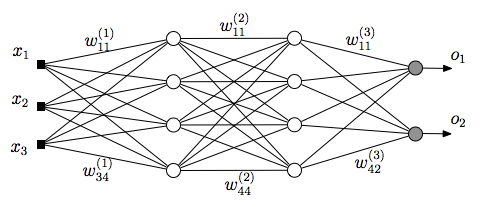
\includegraphics[scale=0.5]{img/MLP}
%     \caption{Paveikslėlio pavyzdys}
%     \label{img:mlp}
% \end{figure}


% \section{Eksperimentinio palyginimo rezultatai}
% % tablesgenerator.com - converts calculators (e.g. excel) tables to LaTeX
% \begin{table}[H]\footnotesize
%   \centering
%   \caption{Lentelės pavyzdys}
%   {\begin{tabular}{|l|c|c|} \hline
%     Algoritmas & $\bar{x}$ & $\sigma^{2}$ \\
%     \hline
%     Algoritmas A  & 1.6335    & 0.5584       \\
%     Algoritmas B  & 1.7395    & 0.5647       \\
%     \hline
%   \end{tabular}}
%   \label{tab:table example}
% \end{table}

\end{document}
